\documentclass[../main.tex]{subfiles}
\begin{document}

\chapter{Triangulierte Graphen}
\label{chapter:trigulated}

Triangulierte Graphen waren eine der ersten Klassen, die als perfekt erkannt wurden. Sie erlauben die Bestimmung der Kliquenzahl und Chromatischen Zahl sowie die Erkennung in linearer Zeit. In diesem Kapitel werden wir den Algorithmus von Fulkerson und Gross kennenlernen, der in verschiedenen Varianten die all diese Resultate liefert.

\begin{definition}
    Ein Graph heißt \emph{trianguliert}, wenn jeder Zyklus im Graphen mit Länge $\geq 4$ eine Sehne \emph{(Chord)} besitzt. Eine Sehne eines Zykluses ist eine Kante, die zwei im Zyklus nicht aufeinanderfolgende Knoten verbindet.
\end{definition}

Eine äquivalente Formulierung ist, das der zyklische Graph $C_n$ für $n\geq 4$ nicht als induzierter Teilgraph vorkommt. Etwas anachronistisch zeigt uns der Starke Perfekte-Graphen-Satz \ref{thm:spgt} damit gleich, das triangulierte Graphen perfekt sind. Um nicht mit Kanonen auf Spatzen zu schießen, zeigen wir die Perfektheit später im Stil von Berge nochmal.

Trianguliert sein ist eine hereditäre Eigenschaft, i.e.: Wenn $G = (V, E)$ ein triangulierter Graph ist, dann ist auch jeder induzierte Subgraph $G_A$ für $A \subset V$ trianguliert.

\begin{figure}[ht]
    \label{fig:trianguliert}
    \centering
    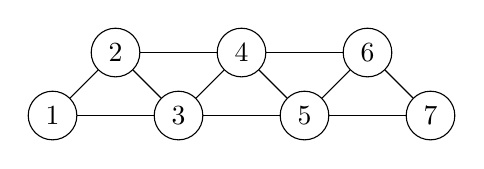
\begin{tikzpicture}[scale=0.8]
        \node[circle, draw] (u1) at (1, 0) {$1$};
        \node[circle, draw] (u2) at (2, 1) {$2$};
        \node[circle, draw] (u3) at (3, 0) {$3$};
        \node[circle, draw] (u4) at (4, 1) {$4$};
        \node[circle, draw] (u5) at (5, 0) {$5$};
        \node[circle, draw] (u6) at (6, 1) {$6$};
        \node[circle, draw] (u7) at (7, 0) {$7$};
        
        \draw (u2) -- (u1);
        \draw (u3) -- (u2);
        \draw (u3) -- (u1);
        \draw (u4) -- (u3);
        \draw (u4) -- (u2);
        \draw (u5) -- (u4);
        \draw (u5) -- (u3);
        \draw (u6) -- (u4);
        \draw (u6) -- (u5);
        \draw (u7) -- (u6);
        \draw (u7) -- (u5);
    \end{tikzpicture}
    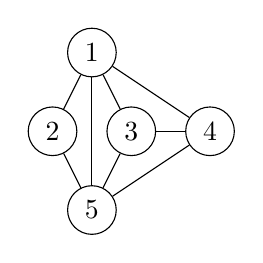
\begin{tikzpicture}[scale=0.5]
        \node[circle, draw] (u1) at (0, 2) {$1$};
        \node[circle, draw] (u2) at (-1, 0) {$2$};
        \node[circle, draw] (u3) at (1, 0) {$3$};
        \node[circle, draw] (u4) at (3, 0) {$4$};
        \node[circle, draw] (u5) at (0, -2) {$5$};
        
        \draw (u2) -- (u1);
        \draw (u3) -- (u1);
        \draw (u4) -- (u3);
        \draw (u4) -- (u1);
        \draw (u5) -- (u4);
        \draw (u5) -- (u3);
        \draw (u5) -- (u2);
        \draw (u5) -- (u1);
    \end{tikzpicture}
    \caption{Beispiele für triangulierte Graphen.}
\end{figure}

\begin{figure}[ht]
    \label{fig:oktaeder}
    \centering
    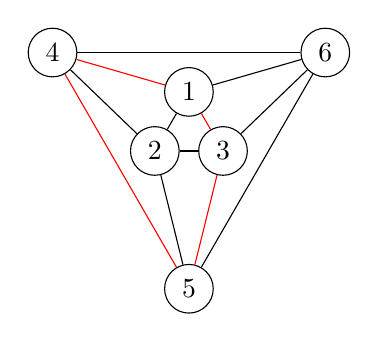
\begin{tikzpicture}[scale=0.5]
        \node[circle, draw] (u1) at (  0+90:1) {$1$};
        \node[circle, draw] (u2) at (120+90:1) {$2$};
        \node[circle, draw] (u3) at (240+90:1) {$3$};
        \node[circle, draw] (u4) at ( 60+90:4) {$4$};
        \node[circle, draw] (u5) at (180+90:4) {$5$};
        \node[circle, draw] (u6) at (300+90:4) {$6$};
        
        \draw (u1) -- (u2);
        \draw (u2) -- (u3);
        \draw [red] (u3) -- (u1);
        \draw [red] (u4) -- (u5);
        \draw (u5) -- (u6);
        \draw (u6) -- (u4);

        \draw (u1) -- (u6);
        \draw [red] (u1) -- (u4);
        \draw (u2) -- (u4);
        \draw (u2) -- (u5);
        \draw [red] (u3) -- (u5);
        \draw (u3) -- (u6);
    \end{tikzpicture}
    \caption{Der Oktaeder-Graph ist kein triangulierter Graph, da der rot markierte Zyklus keine Sehne besitzt.}
\end{figure}

\begin{bemerkung}
    Triangulierte Graphen sind nicht Dreieck-Mesh-Graphen zu verwechselen, wie man sie zum Beispiel aus der Computergrafik kennt. Der Oktaeder-Graph (siehe Abbildung \ref{fig:oktaeder}) besteht nur aus Dreiecken, ist aber nicht trianguliert.
\end{bemerkung}

Wir wollen zunächst eine Charakterisierung der Trianguliertheit über Knoten-Seperatoren beschreiben:

\begin{definition}\label{def:seperator}
    Für einen Graphen $G = (V, E)$ und zwei Knoten $a, b \in V$ nennen wir eine Menge $S \subset V$ einen \emph{Knoten-Seperator} oder \emph{$a$-$b$-Seperator}, wenn der induzierte Subgraph von $V \setminus S$ in zwei (oder mehr) Kompenenten zerfällt und $a$ und $b$ in verschiedenen Komponenten sind.
    
    Wenn keine echte Teilmenge von $S$ selbst ein $a$-$b$-Seperator ist, dann nennen wir $S$ einen \emph{minimalen Knoten-Seperator}.
\end{definition}

% Thm 4.1 Teil 1
\begin{satz}\label{thm:triangulated--completeSeperator}
    Sei $G$ ein ungerichteter Graph. $G$ ist trianguliert, genau dann wenn jeder minimale Knoten-Seperator einen vollständigen Teilgraph induziert.
\end{satz}
\begin{proof}
    $\Leftarrow$: Sei $[a, x, b, y_1, \hdots, y_k, a]$ ein Zyklus in $G$. Es ist zu zeigen, das dieser eine Sehne besitzt. Fall 1: $a$ und $b$ sind verbunden, dann ist $ab$ eine Sehne. Fall 2: $a$ und $b$ sind nicht verbunden. Sei $S$ ein minimaler Knoten-Seperator zwischen $a$ und $b$. Der Knoten $x$ muss auf jeden Fall in $S$ sein, da sonst $a$ und $b$ durch $S$ nicht separiert werden. Ebenso muss eines der $y_i$ in $S$ sein. Da $S$ laut Vorraussetzung vollständig ist, sind $x$ und $y_i$ verbunden, und damit ist $xy_i$ die gesuchte Sehne.

    $\Rightarrow$: Sei $S$ ein minmaler $a$-$b$-Seperator und $G_A$ und $G_B$ die Komponenten von $G_{V \setminus S}$, in denen sich $a$ und $b$ jeweils befinden. Seien $x, y \in S$. Es ist zu zeigen, dass $x$ und $y$ verbunden sein. Da $S$ minimal ist, muss jeder Knoten $x \in S$ einen Nachbaren in $A$ und einen Nachbaren in $B$ haben. Man kann also einen Pfad von $x$ nach $y$ durch $A$ finden. Konkret sei $[x, a_1, \hdots, a_k, y]$ ein kürzester Pfad in $G_{A \cup S}$ mit $a_i \in A$ für alle $i$. Analog sei $[x, b_1, \hdots, b_h, y]$ ein kürzester Pfad in $G_{B \cup S}$ mit $b_i \in B$ für alle $i$. Die beiden Pfade kann man nun zu einem Zyklus in $G$ zusammenbauen: $[x, a_1, \hdots, a_k, y, b_h, \hdots, b_1, x]$ muss laut Vorraussetzung also eine Sehne besitzen. Wo kann sie sein?
    
    \begin{itemize}
        \item Nicht zwischen einem $a_i$ und $b_j$, da $S$ ein Knoten-Seperator ist.
        \item Nicht zwischen zwei $a_i$ und $a_j$ oder einem $a_i$ und $x$ oder $y$, da der Pfad in $G_{A \cup S}$ kürzestmöglich ist.
        \item Analog für $b_i$ und $b_j$.
    \end{itemize}
    Es bleibt also nur die Möglichkeit zwischen $x$ und $y$, was zu zeigen war.
\end{proof}
        
\begin{definition}
    Simplektischer Knoten: Ein Knoten $u$ heißt \emph{simplektisch} (\emph{simplical}), wenn seine Nachbaren alle untereinander verbunden sind, i.e. $adj(u)$ ist eine Clique.
\end{definition}

% Lem 4.2 [Dirac 1961]
\begin{lemma}\label{thm:4.2}
    Jeder triangulierter Graph $G = (V, E)$ hat einen simplektischen Knoten. Wenn $G$ nicht vollständig ist, dann hat $G$ sogar zwei nicht benachbarte simplektische Knoten.
\end{lemma}
\begin{proof}
    Wenn G vollständig ist, dann ist jeder Knoten simplektisch und die Aussage ist trivial. Sonst beweisen wir mittels Induktion über die Knoten-Anzahl:
    
    Induktionsanfang: Ein einzelner Knoten ist als Graph gesehen vollständig.
    
    Induktionsschritt: Sei also $G$ nicht vollständig, also existieren zwei nicht benachbarte Knoten $a$ und $b$. Sei $S$ ein minimaler Knoten-Seperator für $a$ und $b$. Die Komponenten von $G_{V \setminus S}$, die $a$ und $b$ enthalten nennen wir jeweils $G_A$ und $G_B$. Nun nutzen wir die Induktionsvorraussetzung auf $G_{A \cup S}$: Entweder $A \cup S$ ist vollständig, dann ist jeder Knoten in $A$ simplektisch, oder es exitieren zwei simplektische nicht benachbarte Knoten in $A \cup S$ und es können nicht beide in $S$ sein, da $S$ laut Lemma [[[vorher]]] vollständig ist. In jedem Fall existiert ein simplektischer Knoten in $A$ und analog in $B$ auch. Diese sind nicht benachbart, da $A$ und $B$ getrennte Kompnenten sind.
\end{proof}
    
Der vorherige Satz lässt uns auf einen ersten Algorithmus zum Erkennen von triangulierten Graphen schließen: Man suche nach simplektischen Knoten und entferne diese iterativ. Wenn immer simplektische Knoten gefunden werden können, bis der Graph leer ist, dann ist der Graph trianguliert. Wenn in einem Schritt kein simplektischer Knoten gefunden werden kann, dann ist der Graph nicht trianguliert.

Die Reihenfolge, in der man die Knoten entfernt nennt man ein perfektes Knoten-Eliminationsschema (PKE). Konkret ist eine Anordnung aller Knoten von $G$ namhaft $\sigma = [u_1, \hdots, u_n]$ genau dann ein PKE, wenn $\forall i : u_i$ ist simplektisch in $G_{\{u_i, \hdots, u_n\}}$.

%Thm 4.1 Teil 2
\begin{satz} \label{thm:tri_PKE}
    Sei $G = (V, E)$ ein Graph. Dann ist $G$ trianguliert, genau dann wenn $G$ ein perfektes Knoten-Eliminationsschema besitzt. Insbesondere kann jeder simplektischer Knoten ein perfektes Knoten-Eliminationsschema starten.
\end{satz}
\begin{proof}
    $\Rightarrow$: Aufgrund von Lemma \ref{thm:4.2} hat $G$ einen simplektischen Knoten $u \in V$. Der induzierte Subgraph $G_{V \setminus \{u\}}$ ist ebenfalls trianguliert und hat nach Induktion über Knotenanzahl ein perfektes Knoten-Eliminationsschema. Wenn man $u$ vorne an dieses anhängt, hat man ein perfektes Knoten-Eliminationsschema für ganz $G$.
    
    $\Leftarrow$: Sei $C$ ein Zyklus in $G$. Es ist zu zeigen, das $C$ eine Sehne hat. Sei also nach Vorraussetzung ein perfektes Knoten-Eliminationsschema gegeben. Wir nennen den Knoten in $C$ mit dem kleinsten Index im PKE $u$. Die beiden Nachbaren von $u$ im Zyklus werden erst nach $u$ im PKE enfernt und sind verbunden, da $u$ an diesem Punkt im PKE simplektisch ist. Sie bilden also eine Sehne.
\end{proof}    
    
Auf obige Weise ein PKE zu finden funktioniert zwar, ignoriert aber die Tatsache, das uns Satz \ref{thm:4.2} zwei simplektische Knoten liefert. Hier kommt die Idee von Fulkerson und Gross ins Spiel. Da es immer zwei simplektische Knoten gibt, könnten wir uns einen Knoten $u$ zu Beginn aussuchen und für den Schluss aufheben. Falls $u$ einer der beiden gefundenen simplektischen Knoten ist, entfernen wir stattdessen einfach den anderen. Desweiteren können wir uns einen Nachbaren $v$ von $u$ aussuchen, den wir uns für die vorletze Stelle im PKE behalten, da Satz \ref{thm:4.2} nicht benachbarte simplektische Knoten garantiert.

Tatsächlich können wir das ganze PKE von hinten aufbauen.





Besserer Algo von Fulkerson-Gross

zz
LexBFS => L3

zz? (oder nur das)
MCS => L3

zz
L3 Condition + Trianguliert => PKE

zz
LexBFS == PKE <=> Trianguliert
bew: "=>" \ref{thm:tri_PKE}
"<=" Vorherigen beiden Sätze

Dessen Timecomplexity

Triangulated Graphs are Perfect

Schneller Algo um Chomatische Zahl und maximale Cliquen zu finden

\end{document}